\centerline{\bf \Huge А что если Олимпиада сейчас?}
\title{А что если Олимпиада сейчас?}
\begin{flushright}
    \scriptsize Вы все уже победители
\end{flushright}

\problem{1} Запишите десять раз число 1,11 и одиннадцать раз число 1,01. Зачеркните одно или несколько чисел так, чтобы сумма оставшихся чисел была равна 20,19.

\problem{2} Расположите на плоскости точки A, B, C, D и E так, чтобы можно было указать ровно восемь треугольников с вершинами в отмеченных точках. Перечислите эти треугольники.

\problem{3} В поезде 18 одинаковых вагонов. В некоторых вагонах свободна ровно половина мест, в некоторых других — ровно треть мест, а в остальных заняты все места. При этом во всём поезде свободна ровно одна девятая всех мест. В скольких вагонах все места заняты?

\problem{4} У бабушки в саду созрели яблоки: антоновка, грушовка и белый налив. Если бы антоновки было втрое больше, то суммарное количество яблок выросло бы на 70\%. Если бы втрое больше было грушовки, то оно выросло бы на 50\%. На сколько процентов изменилось бы суммарное количество яблок, если бы втрое больше было белого налива?

\problem{5} У Веры есть 27 кубиков с ребром 1 см: 9 красных и 18 синих. Она сложила из них куб с ребром 3 см. Может ли на поверхности куба количество красных квадратиков со стороной 1 см равняться количеству таких же синих?

\problem{6} В каждой клетке квадрата размером 5 × 5 клеток провели ровно одну диагональ. Вершина клетки свободна, если она не является концом никакой из проведённых диагоналей. Найдите наибольшее возможное количество свободных вершин.

\problem{7} Числитель и знаменатель положительной дроби — натуральные числа. Если числитель увеличить на 3, а знаменатель — на 2, то значение дроби уменьшится. Приведите пример и покажите, как такое могло произойти.

\begin{wrapfigure}{r}{0.4\textwidth}
\centering
    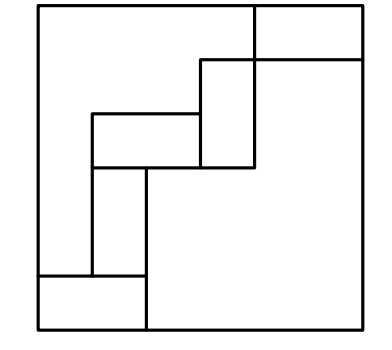
\includegraphics[width=0.15\textwidth]{Сборы Элиста 2023/pict.png}
    \label{fig:Сборы Элиста 2023/pict.png}
\end{wrapfigure}

\problem{8} Пять равных прямоугольников помещены в квадрат со стороной 18 см так, как показано на рисунке. Найдите длины сторон прямоугольника.

\problem{9} На лесопилку привезли трёхметровые и четырёхметровые брёвна. Их распилили на метровые куски, причём каждым распилом пилили ровно одно бревно. Сколько сделано распилов, если вначале было тридцать брёвен суммарной длины сто метров?

\newpage

\problem{10} Четыре седьмых класса поехали на экскурсию. Когда 7А и 7Б пошли в музей, а 7В и 7Г — обедать в кафе, Марья Ивановна подсчитала, что в музее на 15 семиклассников больше, чем в кафе. А когда вечером 7А и 7В пошли в парк, а 7Б и 7Г — в театр, Марья Ивановна насчитала в парке на 8 семиклассников меньше, чем в театре. Умеет ли Марья Ивановна считать? 

\problem{11} Нарисуйте шесть лучей так, чтобы они пересекались ровнов четырех точках, по три луча в каждой точке. Отметьте началалучей жирными точками.

\problem{12} Пять подружек Соня, Таня, Лена, Галя и Вика родились в пяти городах: Риге, Пензе, Казани, Белгороде и Москве. Каждая из них любит конфеты, производимые в одном из этих городов. Известно, что никто не любит конфеты, произведенные в родном городе. Соня любит конфеты из Риги. Таня родом из Риги, у нее любимые конфеты из Пензы. Вика любит конфеты из Москвы. Галины любимые конфеты производят в Белгороде. Вика родом из Казани. Уроженка Пензы любит конфеты, сделанные на родине Лены. Кто из подруг родился в Москве?

